\documentclass{article}
\usepackage{amsmath}
\usepackage{graphicx}
\title{Results}

\author
{
    Dereck Piché \and
    Jonas Gabirot \and
    Guillermo Martinez\and
}

\begin{document}
\maketitle
\section{Summary}
\section{Introduction}
\subsection{Context}
Nucleic acid structures such as DNA (Deoxyribonucleic acid) and RNA (ribonucleic acid) are the foundation of life.
However, these structures are themselves a linear combination of 4 types of nitrogenous bases: A (Adenine), G (Guanine), C (Cytosine) and T (Thymine, in the case of DNA).
In their simplest form, DNA molecules can be conceived as single-stranded, one-dimensional, linear sequences of nitrogenous bases, which are commonly referred to as oligonucleotides.
When synthetized in a way as to possess affinities, these oligonucleotides are referred to as aptamers.
Every aptamer is the result of a SELEX (Systematic evolution of ligands by exponential enrichment) procedure in which those possessing binding affinities towards specific molecules are recursively selected and reproduced by the experimentalist.
Consequently,  aptamers are a promising biotechnology and have been found useful for tracking the propagation of various molecules in their respective environments such as pathogens, toxins, antibiotics and pesticides in food, water and soil samples (Dunn et al., 2017), as well as adenosine triphosphate in cells (Zhang et al., 2019).

Similar to other DNA molecules, single-stranded aptamers fold into two-dimensional structures, and eventually three-dimensional structures, through base pairing interactions among themselves or with other aptamers.
At specific temperatures and ionic concentrations, higher dimensional aptamer structures display specific levels of free energy. The lower the entropy, the lower the free energy of the molecule.
The lower the free energy, the higher the stability of the folded aptamer structure. Pipelines such as NUPACK can predict the change in free energy between the higher and lower-dimensional configurations of a given aptamer— a given one-dimensional sequence of nitrogenous bases.
The more negative the variation in free energy (indicating that the higher dimensional state of the aptamer minimized the free energy of its one-dimensional state), the more stable the folded structure of a single-stranded aptamer is predicted to be.

There is a trade-off between binding affinity and folded stability. Longer DNA sequences tend to be more stable, whereas shorter sequences tend to possess higher binding affinity.
We hypothesize that 30 bases-long aptamer sequences will be a good compromise.


\subsection{Motivation}
The purpose of this research is therefore to train deep learning neural 
networks with randomly generated DNA sequences to predict the minimum 
free energy structure given by ‘NUPACK’.
The most stable aptamer sequences will be potential candidates to 
undergo the entire E2EDNA protocol and be tested on their binding 
affinity to a wide range of analyte of interest. The aptamers that 
are the most stable and possessing the highest binding affinity will 
be potential candidates to be synthetized and used to solve specific 
problems such as trace the oil molecules in the oceans after a spill. 
Given that shorter random-sequence libraries of doubly modified aptamers 
usually posses a higher binding affinity for a target than larger 
traditional sequences (30-mer VS 40-mer random regions), the length 
of our random sequences will be of 30-mer (Dunn et al., 2017). 
\section{Summary}
\section{Litterature Review}
There is currently little research and writing on learning 
aptamer properties with deep learning algorithms. Instead, biology-specific algorithms 
biology-specific algorithms are favoured, as well as clustering algorithms. 
clustering algorithms. For example, this article from January 2023 uses 
an original algorithm that combines clustering methods to find an optimal 
an optimal aptamer from a selection. 
https://pubs.acs.org/doi/pdf/10.1021/acssynbio.2c00462.
However, some recent papers use deep learning. 
"Machine learning guided aptamer refinement 
and discovery" (https://www.nature.com/articles/s41467-021-22555-9) 
uses a standard MLP neural network to find the most compatible (high affinity) aptamers with target molecules. The estimation of free energy is a sub-step of the affinity calculation. It performs a 
truncation step to minimise the length of the aptamer without altering its properties. 
Another deep learning model with aptamers is AptaNet 
(https://www.nature.com/articles/s41598-021-85629-0). This model uses an 
MLP and a CNN to learn the relationship between aptamers and target proteins 
proteins (Aptamere-protein relations or API). The MLP works best, with a 
test accuracy of 91.38%. This neural network performs significantly better than more traditional 
algorithms such as SVM, KNN and random forests. However, this model 
uses a very detailed database containing numerous auxiliary variables 
measured in the laboratory for each individual, but with only 1000 individuals. 
No published aptamer model uses transformers or RNNs to predict free energy, so the 
predict free energy, so our method would be original in this field.

\section{Methods}
Let us briefly resume our task once again in order to make this document
self-contained. Our task is to create models capable of reproducing 
the classical algorithms used by the NUPACK foundation to predict the 
free energy ($\in R$) of a DNA strand (a sequence of the elements of $\{A,C,G,T\}$).
\section{Planned Methodology}
\subsection{Training dataset}
First, we will have to generate our training data. We shall implement a 
simple python script which uses the NUPACK python library in order
to generate a .json file containing our training data. We  
will generate a dataset of a $1,000,000$ random DNA strands of length $30$, paired with their free energy as calculated by NUPACK. In the event that this dataset does not not
suffice for adequate prediction accuracy (according to mean squared error), we will
generate more examples and augment the expressivity of our models.
\subsection{Baseline Algorithms}

\subsubsection{Multilayered Perceptron}
A multilayer perceptron (MLP) is a type of artificial neural network that consists of multiple layers of interconnected nodes organized into an input layer, one or more hidden layers, and an output layer. Each node in the MLP receives input signals from nodes in the previous layer, applies a non-linear activation function, in our case ReLU, to the weighted sum of those inputs, and passes the resulting output signal to nodes in the next layer. The weights between the nodes are learned through a process called backpropagation, where the network adjusts its internal parameters to minimize the difference between its predicted outputs and the actual target outputs. MLPs are widely used for supervised learning tasks such as classification and regression, and have been applied in areas such as computer vision, speech recognition, and natural language processing. Unlike transformers and RNNs, MLPs make no assumption about the sequential nature of the input data. In this way, an MLP is a more general algorithm and is thus well-suited to be a baseline comparison to test our assumptions about the data. For preliminary testing, we shall use an MLP with 10 hidden layers and an input size of 120, (30 bases of DNA one-hot encoded). We shall use the Adam optimizer as it is the most commonly used optimizer.

\paragraph{Cost Function}
Since this is a regression task, we shall use the Mean Squared Error (MSE) as the loss function.

\paragraph{Encoding}
To feed a string input to an MLP, we shall convert each base (A,C,T,G) to a one-hot encoded vector. With 4 categories and sequences of length 30, this gives an input size of 120.


\subsubsection{Decision trees with AdaBoost}
We might want to use this as a baseline. 


\subsection{Advanced Algorithms}

\subsubsection{Recurrent Neural Network}
Recurrent neural network (RNN) is a deep lRecurrent neural network 
(RNN) is a deep learning architecture used for sequential data prediction
using both current and past inputs. earning architecture used for sequential 
data prediction using both current and past inputs. 

it in a simple way, RRN architectures are composed of an encoder and a encoder. The initial input is vectorized by the encoder and processed as a function of the initial state, which is random at first. As a result, the encoder's weights and biases are adjusted in the form a second state to incorporate both current and past input information. The encoder recursively processes the following vectorized inputs as functions of current states, while updating the weights and biases of current states to produce new states at each iteration. The encoder terminates this recursion when it has iterated over an entire sequence of features and concludes by transmitting its final state, which incorporates all previous states, to the encoder. In the case of a many-to-one RNN underlying architecture, this paper's architecture of interest, the encoder produces one output prediction as a function of the final state received from the encoder and as a function of its own current state, random at first. By contrasting the predicted output value to the actual value of the sequence, the encoder performs gradient descent to minimize the loss function, updates its current state and backpropagates it to the encoder's states. Once the weights and biases of the encoder states are adjusted, it iterates over the following sequence of features following the same recursion procedure. This recursive process is repeated for the entire length of sequences within the training set, and the regression model is cross-validated on its ability to minimize the squared mean error between target and predicted output values in the validation and test set. 
\begin{figure}
    \caption{Illustration of RNN architecures}
    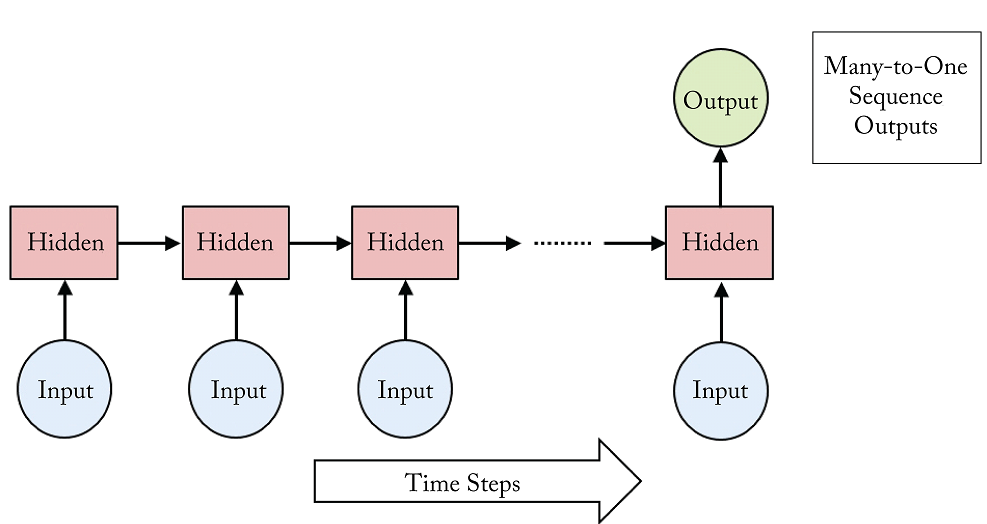
\includegraphics[width=0.7\textwidth]{images/2023-03-17-16-42-13.png}
\end{figure}

RNNs are not without challenges. In order to update parameters, the backpropagation algorithm needs to calculate gradients at each different step. This usually results in unstable neural networks due to vanishing and exploding gradients which are unable to learn long-term dependencies. Long Short Term Memory networks (LSTMs) have been proposed to avoid these problems and designed to handle long-term dependencies. Initially proposed by Hochreiter and Schmidhuber (1997) \cite{hochreiter1997long},  LSTMs use cells with input, output and forget-gate to control the flow of information. 
\begin{figure}
    \caption{Long Short Term Memory cell}
    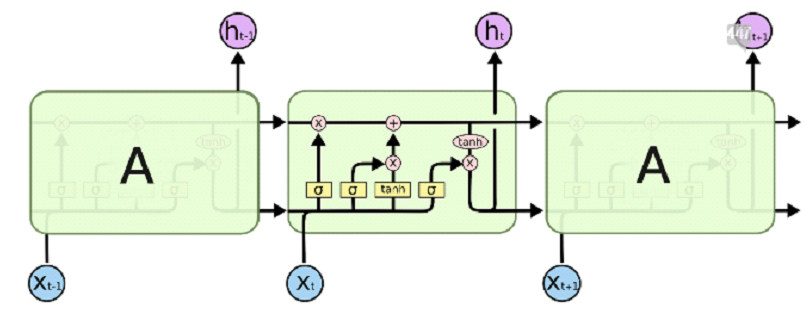
\includegraphics[width=0.7\textwidth]{images/2023-03-17-16-38-22.png}
\end{figure}



Given this paper's task to predict the level of free energy given a sequence of 30 features, we will train a many-to-one LSTMs for a regression task with multiple input time series. We will divide our entire dataset in training $80\%$, $10\%$ for testing and $10\%$ for validation. For each training instance, we will give the model a sequence of observations and a corresponding target value. The goal will be to forecast time series' free energy within the validation set. Time given, hyperparameter tuning will be performed on the validation set to optimize the choice of the learning rate, the number of units or layers, and the weight regularization techniques used as penalties on the loss function. Finally, the tunned model's prediction accuracy will be calculated on the test set using Mean Squared Error (MSE) and Mean Absolute Error (MAE) metrics. 
\begin{figure}
    \caption{Information flow}
    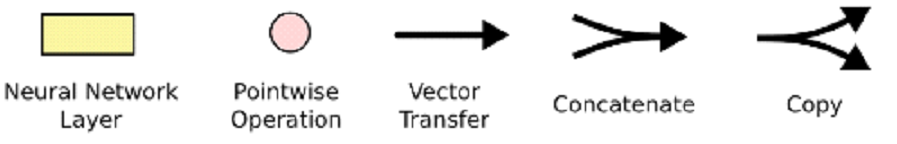
\includegraphics[width=0.7\textwidth]{images/2023-03-17-16-41-25.png}
\end{figure}

\subsubsection{Tranformer}
\paragraph{Architecture}
The transformer architecture was initially made to translate text.
However, it's subsequent use was mostly tied to token generation. 
This use only required the encoder to be part of the architecture, 
and recursively fed the predicted token in the current input while 
truncating if the input size was over the limit.
Our task is vastly different. We are dealing with a regressive task,
since we are trying to learn a function of the form $R^n \to R$.
Thus, we shall only keep the encoder part of the transformer architecture. 

We shall use a simple linear mapping of the encoder output to the reals.
If this approach is note successfull, we will consider adding a more complex
network to replace the linear mapping.
\paragraph{Cost Function}
Since this is a regressive task, we shall use various instances of the 
$l_p$-norm as our cost function.

\paragraph{Tokenisation, encoding, positionnal encoding}
Since the tranformer learns the embedding in the attention heads\cite{transformers}, 
we shall simply use an integer mapping for the set of tokens $\{A,C,G,T\}$ as opposed to 
one-hot encoding. This is done partly due to the way the Pytorch library works.

On top of the embedding layer, we will add a positionnal encoding, which as the
name suggests, transforms the input values in such a way that positionnal information 
is implicitely given in their structure. There are many ways to do this. At first, we will use 
a template created by Pytorch and available in their documentation which creates
a positionnal using $sin$ and $cos$ functions (the code will be copied and 
pasted directly without modifications). If this positionnal encoding does not
work well, we shall implement one of our own.

We will train and compare the accuracy of our encoder-only tranformer with 
respect to the absence and inclusion of positionnal embedding to the input tokens.



\paragraph{Advantages}
What makes the encoder-only transformer different from other models? What are
we taking advantage of by it's use? As opposed to recurrent neural networks, 
this model is less sequential in nature. We are predicting by 
taking the sequence of tokens all at once. We have high hopes for the 
distributivity of attention made possible by the head multiplicity.
We can imagine that there is high importance between the ends of the DNA 
sequence, and at the center. A transformer, given enough data, would 
be able to take advantage of this structure in order to simplify the task.


\subsection{Comparisons and analysis}
It would be more logical to compare learned models with a similar 
number of parameters. This would give us more information as 
to if the comparative advantages were caused by the particularities 
of the architecture or simply because of the increase of expressivity 
tied to bigger models. Our analysis will make extensive use of graphical 
representations of the evolutions of the loss with respect to the number 
of epochs performed during training. We will use the same number 
of training examples for each model, though we do not plan on keeping 
the order of training batches nor the particular elements of the training 
batches equivalent.

\subsection{Results}
\section{Results}

\paragraph{MLP} Our MLP with 20 hidden layers and 1 million parameters trained on 90\% of the data set and tested on 10\% achieved a test MSE of 0.94, which is quite poor.

\paragraph{LSTM} Our LSTM with 1 million parameters trained in the same way achieved a very similar test loss of 0.91 before starting to overfit.

Both of these architectures had their hyperparameters fine-tuned extensively to find an acceptable result, but neither of them worked.

\paragraph{Transformer} We then implemented a transformer architecture modified to work on a regression problem. Although this model was bigger at 1.8M parameters, it achieved much better results, ending with a test loss of 0.15, a very promising result.

All models were trained by intervals of 10 epochs, until they started overfitting. They were not stopped at the same time. The evolution of the losses of the models can be seen in the annex.


\paragraph{Scaling} Given the small size of our model, the small size of our dataset and the know scaling properties of transformer models, the promising result of our transformer indicates that we may achieve near-perfect prediction of free energy with a larger set of training examples and a larger model.

\paragraph{Larger Model} To test this hypothesis, we trained a larger transformer model with 8M parameters (about 4 times bigger), on the same dataset. It achieved a test MSE of 0.12, a slightly better result. This represents a 20\% reduction of the Mean Squared Error compared to the smaller model. However, this model was not fine-tuned due to lack of time. We were also unable to test our transformer model on a larger dataset due to lack of time.


\paragraph{Analysis} To better understand the strengths and weaknesses of our large transformer model, a more thorough analysis of its predictions follows:

Note: Because the model overfitted before the weights were saved, the MSE for this analysis is 0.15, as opposed to the better result of 0.12 that was mentioned earlier.

On average, our model underestimates the free energy of a strand by 0.27 and the variance of its predictions is 24\% higher than that of the true values. For further analysis, our results were split into four quarters, going from the lowest free energy label to the highest one. The lowest quarter had the worst performance, with a MSE of 0.35. The second lowest was similar to the overall result, with a loss of 0.15. The second highest had a much better result, with a MSE of 0.08, and the highest one was even better at 0.03. These numbers show that our model performs much better on strands with high free energy.

A graph of the distribution of the free energy labels in our dataset and an analysis of its variance shows that it is skewed towards high free energy values, thus the variance in high free energy strands is much lower than in low free energy strands. This means that for each high energy strand, the model has trained on many more strands with a similar free energy than it has for a lower energy strand. This suggests that increasing the number of training examples would greatly increase the performance of our model, in particular if they are filtered to make a more uniform distribution of free energy labels in the training dataset.
\subsection{Conclusion}
\subsection{Contributions of Each Member}
\subsection{References}
\end{document}